

\section{SONAR and Sound Analysis an Introduction}

\subsection{Background}

For submariners, the ability to detect the presence of surface ships and other submarines while remaining undetected is a matter of life and death. To achieve this, passive SONAR detection techniques have been developed to detect, classify, and determine target speed based on noise emissions. Often, detection is made harder when the signal from the ship is lost in background noise. This can occur when the marine environment is particularly noisy and/or when the ship is distant from the submarine. In order to maintain contact with a target vessel, detection must rely on some form of signal processing to enhance the acoustic signature of the ship and reduce the impact of the background noise in the sonar signal.

Remarkably, the developers of MNW have included sophisticated in-game representations of the principal components that make up the core of the detection and classification tools. These tools can only be representative of those actually used as most are classified secret by navies around the world; though, it is surprising how much is available in the public domain. Some key references are listed in the \hyperref[sec:References]{references section}. The developers have set an ambitious target of achieving as near-realistic sound modelling and propagation as is possible for the capabilities of a reasonably spec'd PC with a modern GPU. Using GPU ray-tracing capabilities, the mechanics of sound movement in water are accurately modelled. For those with long memories you will be familiar with rudimentary versions of these tools in submarine simulations such as EA's Sub Command and Black Bean's Dangerous Waters.

The process of capturing, analysing, and final classification of a target is shown in Figure 12. This workflow uses several processes which are explained below. A more detailed discussion is provided in \hyperref[sec:Appendix_B]{Appendix B}. However, for a player of MNW, the information provided in this section provides a sufficient understanding of what MACS and the game's systems are telling you.

\begin{figure}[h]
    \centering
    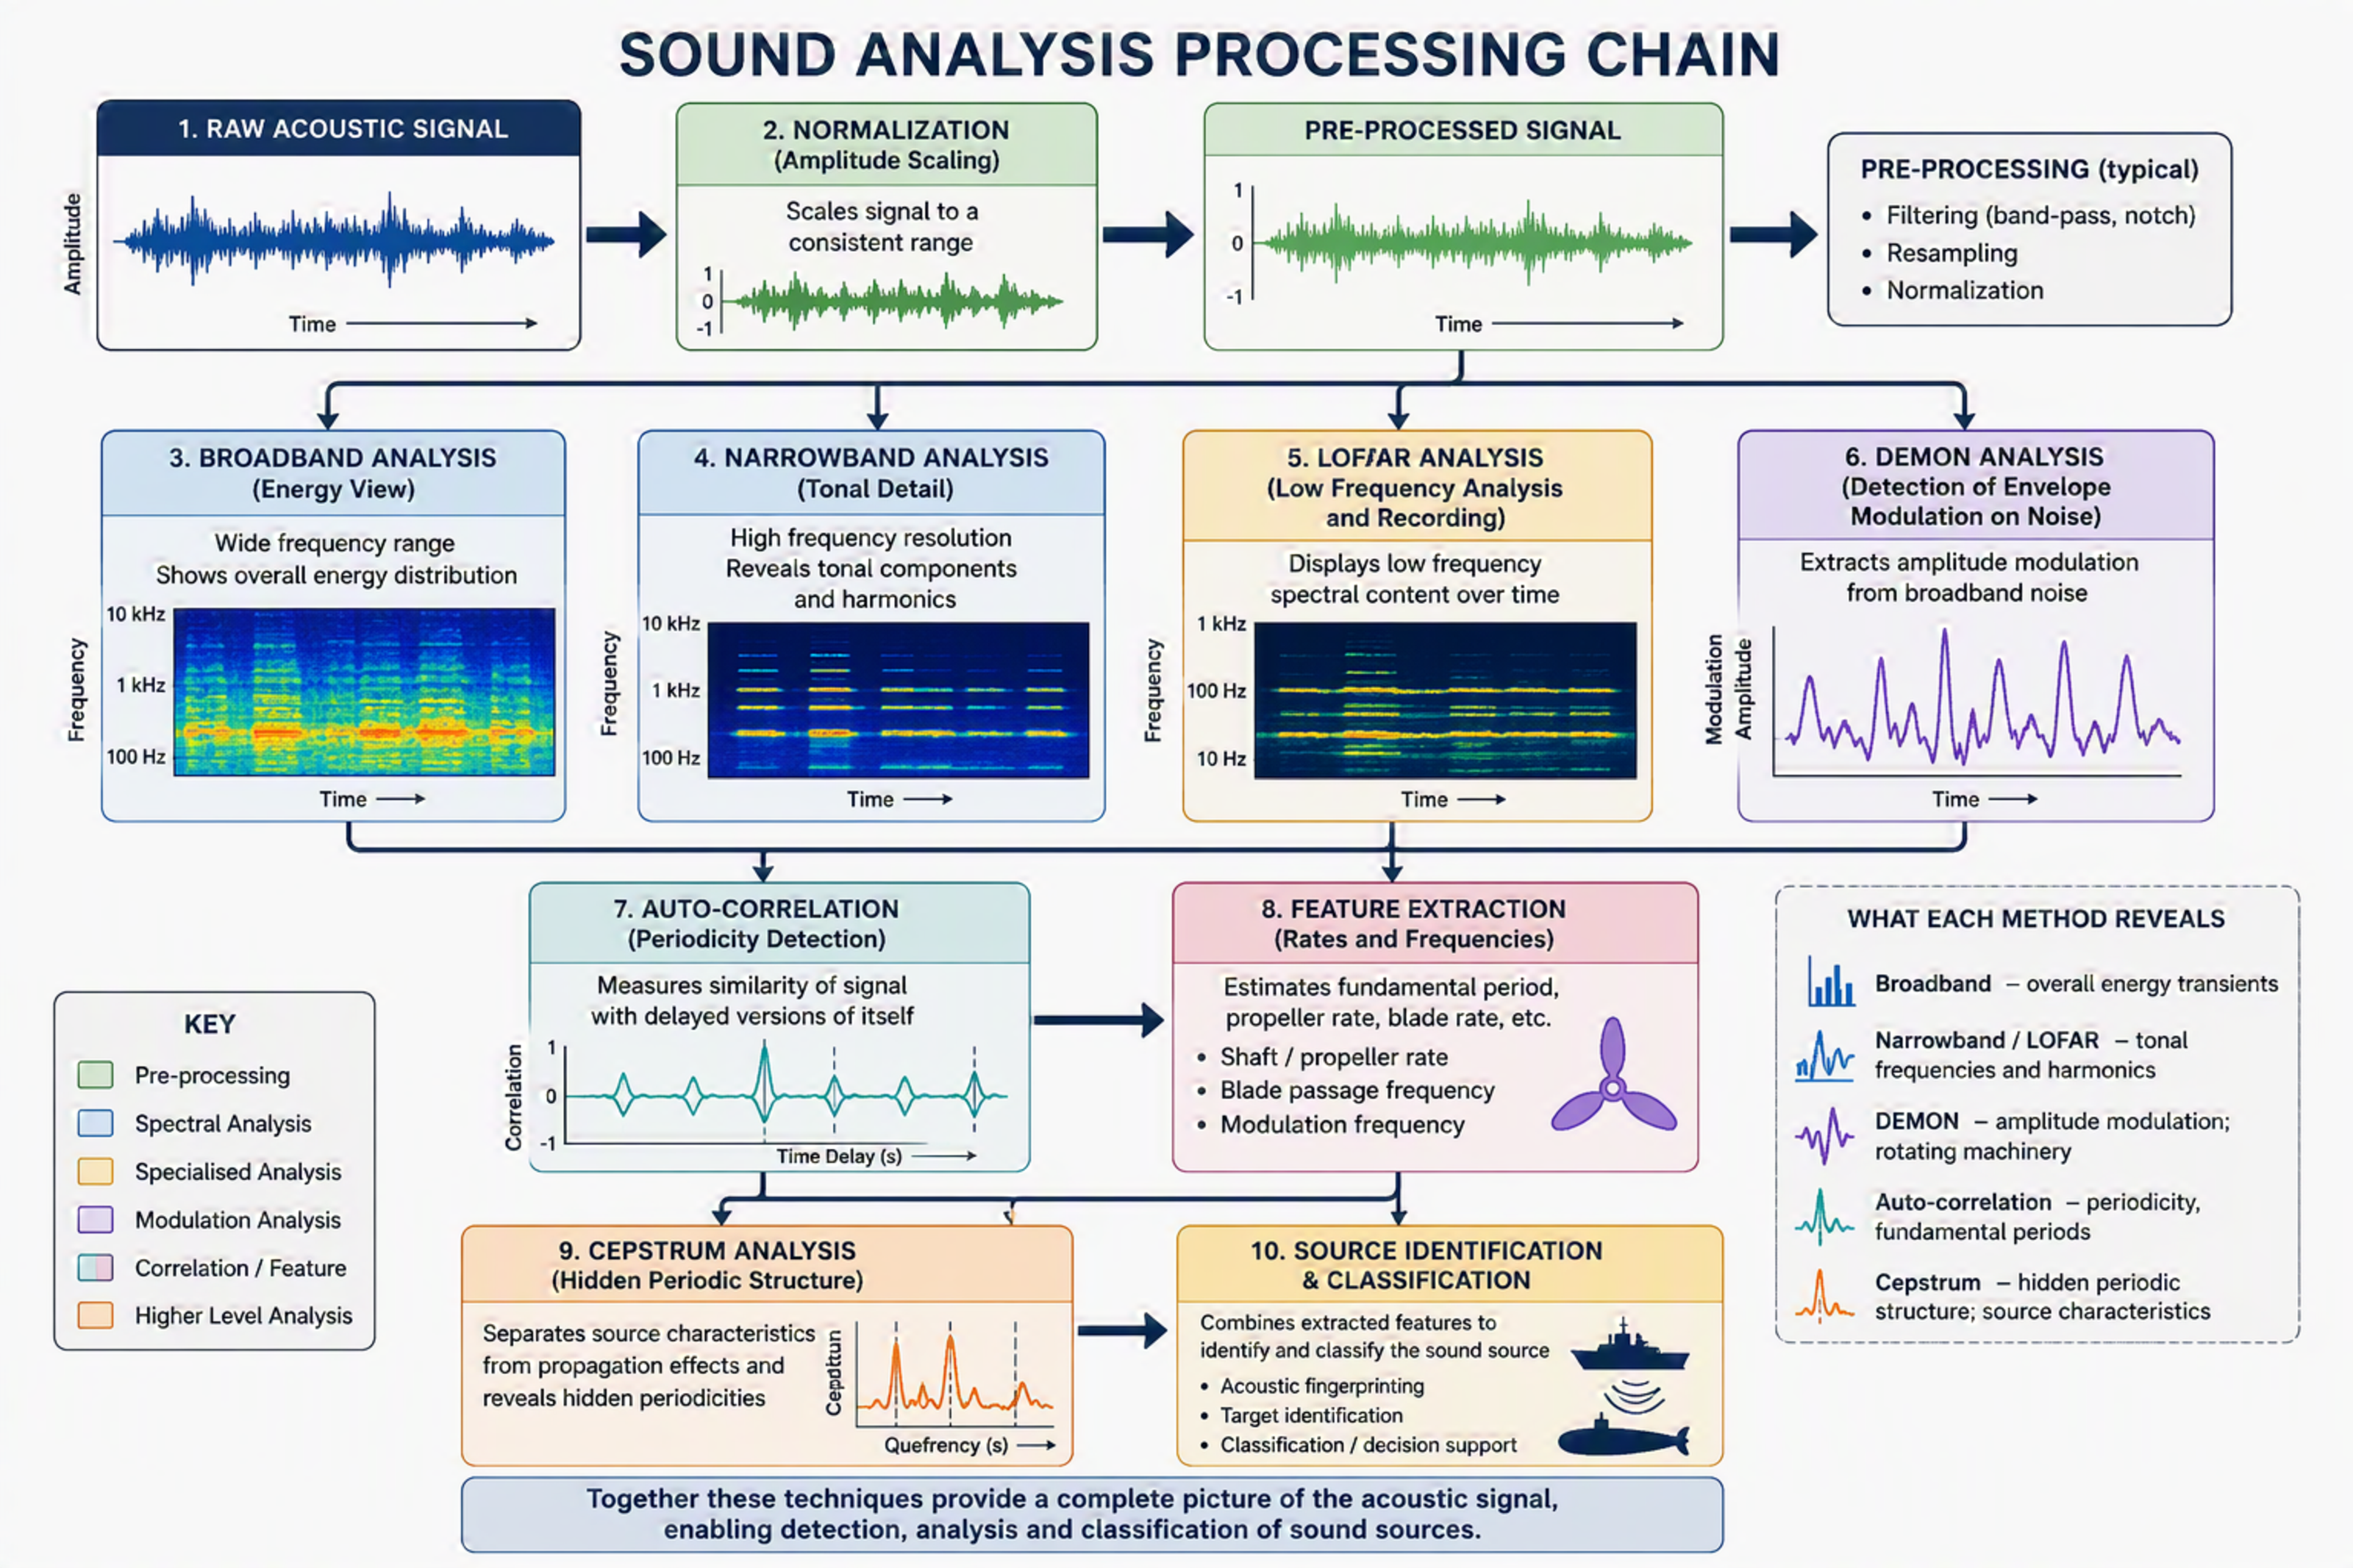
\includegraphics[width=\linewidth]{../img/actuals/sound_workflow.pdf}
    \caption{Sound analysis workflow}
\end{figure}

When MACS is used in conjunction with MNW as designed, the sound has undergone some processing in game so it can be argued that pre-processing is shared between MNW and MACS in this case.

\begin{faintquote}
    Sound analysis is the process of examining acoustic signals to extract useful information about their source, characteristics, and behaviour. Sound signals are often complex, containing multiple frequency components, background noise, and transient events. To understand these signals effectively, a range of signal processing techniques is used.
\end{faintquote}

\subsection{Broadband and Narrowband}

Broadband and narrowband analysis are complementary ways of processing the acoustic energy received by a submarine's sensors. A submarine hunting a target will typically use both methods because each provides different information. In MNW, your principal receivers of sound energy are the bow array (LAB), the flank arrays (WAA), and the two towed arrays (TA), TB34 and TB29A. Broadband analysis examines sound energy across a wide range of frequencies. It focuses on overall acoustic energy rather than specific discrete tones. Broadband is where you will often first see a contact, although this is not always the case. Narrowband analysis, on the other hand, uses finer frequency resolution to reveal detailed spectral features such as harmonics and tonal components produced by machinery, propeller blade rates, or engine harmonics. It does this by applying a Fourier Transform (FT) transforming the sound from a time based domain to a frequency domain (\hyperref[sec:Appendix_B]{Appendix B}). These frequencies are displayed as discrete tonal lines which can often be an identifying fingerprint for the contact.

\textbf{Broadband Strengths}
\begin{compactitem}
    \item \textbf{Long-range detection:} Often provides a first indication of a contact because it collects energy over a wide frequency range.
    \item \textbf{Good against noisy targets:} Effective when a target generates substantial broadband noise from propulsion or hydrodynamic flow.
    \item \textbf{Rapid contact detection:} Useful for searching large areas and finding contacts quickly.
    \item \textbf{Works when tonal lines are weak or absent:} Can detect targets whose machinery tones are masked or difficult to resolve.
\end{compactitem}

\textbf{Broadband Weaknesses}
\begin{compactitem}
    \item \textbf{Limited classification capability:} Indicates that a contact exists, but provides little information about what it is.
    \item \textbf{Vulnerable to environmental noise:} Shipping, sea state, and biologics can create broadband noise that causes false or ambiguous detections.
    \item \textbf{Less precise tracking:} Bearing estimates and contact characterization may be less accurate than narrowband methods.
\end{compactitem}

\textbf{Narrowband Strengths}
\begin{compactitem}
    \item \textbf{Excellent classification and identification:} Tonal patterns can reveal target type and sometimes specific class.
    \item \textbf{Supports tracking:} Stable tones allow accurate bearing tracking over time.
    \item \textbf{Useful against quiet contacts:} Even very quiet submarines may produce detectable tonal signatures.
    \item \textbf{Provides target motion clues:} Changes in tonal frequencies can support Doppler analysis and target speed estimation.
\end{compactitem}

\textbf{Narrowband Weaknesses}
\begin{compactitem}
    \item \textbf{Requires strong, resolvable tonal lines:} If the target is extremely quiet or its tonals are masked, analysis becomes difficult.
    \item \textbf{More susceptible to frequency instability:} Manoeuvering, environmental effects, and machinery changes can complicate interpretation.
    \item \textbf{Generally less effective as an initial search tool:} It often requires an already-established contact bearing.
\end{compactitem}

Imagine a submarine is listening for another submarine transiting at moderate speed. The target's propeller, machinery, flow noise, and other sources create a broad spectrum of noise. Broadband processing may detect a rise in acoustic energy from a particular bearing, suggesting a contact, the operator might see a contact emerge from the background noise even before any specific identifying features are apparent. After broadband analysis detects a contact, operators switch attention to narrowband displays. They may observe a set of stable tones at particular frequencies. Those frequencies can be compared to intelligence databases, acoustic signatures, notebooks and experience.

A weak broadband signal does not always mean weak spectral features. From a broadband point of view a very faint vessel at 50Hz broadband is merged with contributions from a much wider frequency band. This means that BB is dealing with background noise from all of that frequency range. So the signal to noise ration (SNR) is very low or indiscernible on the broadband screen. Narrow band on the other hand looks at how much energy is available at each frequency band (Fourier Transform) and bins them in bands. So in the frequency domain the 50hz signal will stand out and this is reinforced by persistence of the signal over time.

Where broadband may give an early detection is for a good SNR and when enough energy is being pumped into the water. In this case broadband is very effective. A source with strong broadband noise might appear BB-first. A comparatively quiet source with prominent persistent machinery/propulsion tonals can potentially become apparent in NB/LOFAR without an obvious BB signature.

\begin{faintquote}
    In modern anti-submarine warfare, classifiers do not choose one over the other; they use them together. Narrowband data is used to classify the specific ship type via its engine noise, while broadband data (both passive flow noise and active echoes) is used to map the target's size, speed, and exact spatial position.
\end{faintquote}

\subsection{Normalization}

Before advanced analysis is performed, signals are often subjected to normalisation. Normalisation is a statistical technique that scales the signal amplitude to a consistent range. A well-known and commonly used method is the Z-score however there are many other strategies available. The effect is to reduce the influence of recording-level variations, allowing meaningful comparisons between different measurements. This preprocessing step improves the robustness of subsequent analysis techniques and ensures that results reflect the signal characteristics rather than differences in recording conditions. The approach used by MACS to normalise data is explained in \hyperref[sec:Appendix_B]{Appendix B}.

\subsection{LOFAR (Low Frequency Analysis and Recording)}

In underwater acoustics and sonar applications, LOFAR is a fundamental technique. It is a passive narrowband sonar signal-processing technique which displays the spectral content of low-frequency signals over time. These tonal signatures can act as acoustic fingerprints, helping to detect, classify, and sometimes identify ships and submarines from the sounds they radiate into the water. Narrowband is used because:

\begin{compactitem}
    \item \textbf{Extreme Long Range: }Low-frequency narrowband signals can travel very long distances through the ocean without losing energy (\href{https://www.youtube.com/watch?v=sP85wUcg6_A}{YouTube}), allowing for early detection of distant threats.
    \item \textbf{High Signal-to-Noise Ratio: }By filtering out background ocean noise and focusing strictly on ultra-thin frequency bands, LOFAR can extract faint mechanical signals that are otherwise invisible to the naked ear or broadband sensors
\end{compactitem}

\begin{faintquote}
    Below roughly 100 Hz, ocean conditions can allow very efficient propagation with relatively low energy loss, which is why low-frequency sound may travel enormous distances. But the low-frequency ocean is also a very noisy place, with shipping, machinery, environmental noise and other sources contributing substantial energy. That is exactly why "travels further" does not necessarily mean "easier to detect". Sonar performance ultimately depends on received SNR, not merely propagation distance.
\end{faintquote}

Sound received by the SONAR arrays is transformed into a "frequency domain" which shows how much energy exists for every single frequency. This is typically done using a FFT (Fast Fourier Transform). FFT is a mathematical algorithm which allows the huge amount of information contained in the sound data to be analysed quickly. The result is displayed as a LOFARgram (a time-frequency spectrogram), where persistent frequency components appear as lines. This is useful because ships and submarines generate characteristic underwater noise from:

\begin{compactitem}
    \item Main engines and generators
    \item Gearboxes and pumps
    \item Propeller blade rotation and cavitation
\end{compactitem}

These sources produce distinctive frequency components. By examining the pattern of tonal lines in a LOFAR display, operators can distinguish different vessel types and, specific classes of ships and, sometimes, individual ships. To summarize, NB analysis describes the type of spectral analysis, i.e. high frequency resolution separating spectral components that are very close together to reveal distinct tonals. LOFAR is an application and presentation of a narrowband analysis typically focussing on the lower-frequency part of the spectrum as this is where many diagnostic tonals are, e.g. shaft rate, blade rate etc. So, to be concrete NB refers to spectral resolution / bandwidth and LOFAR describes the signal-processing and visualisation techniques.

\begin{faintquote}
    In summary, LOFAR is a passive sonar technique that converts underwater sounds into a time-frequency display, enabling operators to detect ships and identify them from their unique acoustic signatures. LOFAR is often paired with DEMON analysis.
\end{faintquote}

\subsection{DEMON (Detection of Envelope Modulation on Noise)}

DEMON processing focuses on amplitude modulations (AM) present within broadband noise. In simple terms, it means taking a steady, continuous wave and making it rhythmically louder and quieter over time. For example, the rotation of a ship's propeller produces periodic fluctuations in noise levels at characteristic frequencies, such as:

\begin{compactitem}
    \item Shaft rotation frequency
    \item Blade-passing frequency or Blade Rate(BR)  
\end{compactitem}

DEMON extracts the amplitude envelope of the received noise and analyses it in the frequency domain. The resulting spectrum reveals peaks corresponding to the vessel's mechanical and propeller characteristics, which can be used for identification and classification. This is useful because:

\begin{compactitem}
    \item Enhances weak periodic signatures hidden in broadband noise.
    \item Helps estimate propeller speed, number of blades, and other target features.
    \item Widely used in passive sonar target detection and classification systems.
\end{compactitem}

\begin{faintquote}
   \textbf{LOFAR} emphasizes the ship's frequency spectrum (machinery and tonal components). \textbf{DEMON} is useful for extracting propeller-related modulation and blade-rate information. 
\end{faintquote}

\subsection{Cepstrum and Auto-correlation}

\textbf{Cepstrum} analysis is a powerful signal-processing technique used in acoustics. Developed to reveal hidden periodic structures in the frequency spectrum of a signal, it is particularly effective for separating source characteristics from propagation effects.

The basic idea behind cepstrum analysis is to detect echoes, repeating patterns, or modulation effects within a signal. In many real-world applications, a recorded signal is not simply a direct waveform but rather a combination of a source signal and the influence of the medium or system through which it passes. For example, in sonar, received energy may contain reflections from multiple surfaces, and in machinery monitoring, vibration signals are influenced by rotating components and gears. Cepstrum analysis helps separate these effects and identify underlying periodicities.

\textbf{Auto-correlation} is commonly used to detect periodic acoustic signatures produced by ships, submarines, and marine machinery. Many sources generate signals that repeat at regular intervals, such as rotating propellers, diesel engines, pumps, and gear systems. The periodic nature of these sounds produces corresponding peaks in the auto-correlation function. The spacing between peaks indicates the repetition period, from which the rotational speed or blade-passage frequency can be estimated.

In simple terms, auto-correlation measures how similar a signal is to a delayed version of itself. By comparing the signal with progressively shifted copies, it becomes possible to detect hidden periodicities and determine whether certain features repeat over time.

For example, consider a vessel whose propeller completes two revolutions per second. If the acoustic signal generated by the propeller repeats every 0.5 seconds, the auto-correlation function will exhibit peaks separated by approximately 0.5 seconds. The analyst can use these peaks to determine the underlying mechanical characteristics of the vessel and potentially aid in classification and tracking.

You will find more details about Cepstrum and auto-correlation in \hyperref[sec:Appendix_B]{Appendix B}.

\pagebreak